\documentclass[12pt]{article}

\usepackage[a4paper, left=2.5cm, right=2.5cm, top=2.5cm, bottom=2.5cm]{geometry}
\usepackage{times}

\usepackage[style=base, font=small, labelfont=bf]{caption}
\usepackage{subcaption}

\usepackage[backend=biber]{biblatex} %Imports biblatex package
\addbibresource{thesis.bib}

%\renewcommand{\baselinestretch}{1.15}     % Defines the line spacing
%should be setspace package???s

\usepackage{graphics,graphicx,epsfig,ulem}  % Graphics package
\usepackage{svg}
\graphicspath{{../Figures/}}


\usepackage{amsmath} 						% Maths package

%\usepackage{siunitx} % SI units, alignment in tables
%\sisetup{round-mode=figures, round-precision=3}

%\usepackage{lipsum}
%\usepackage[british]{babel} % British date system

%\usepackage{multirow} % Multi-row cells in tables
\usepackage{booktabs} % Nice table separators

%\usepackage{hyperref} % For hyper-references

%\usepackage{float}

% Could make titlepage?
\title{Quantum annealing for music arrangement}
\author{Lucas Kirby\\Department of Physics, University of Durham \and Supervised by\\Dr Robert Potvliege \& Dr Omer Rathore}
\date{23 April 2025}

\begin{document}

\maketitle

\begin{center}
    \includesvg{durham-university.svg}
\end{center}

\vfill

\begin{abstract}              

Music arrangement is usually a complex and time-consuming process; this paper aims to provide an automatic method by which to arrange music via a quantum computing technique called quantum annealing. By splitting a score into a set of phrases, these phrases can form a quadratic unconstrained binary optimisation (QUBO), a function which the quantum computer aims to minimise by choosing the values of discrete variables. At the end of the optimisation process, the resulting chosen values describe the final arrangement, which can then be interpreted into sheet music. This method is tested on an excerpt of Beethoven's String Quartet No. 10 in E-flat major; in this case, the optimisation process is successful, and selects compatible phrases that produce a suitable arrangement. \cite{lucas_ising_2014}

\end{abstract}

\vfill

\clearpage

\tableofcontents

\thispagestyle{empty}

\clearpage

\section{Introduction} 

Music is often seen as a very human endeavour. For centuries, only skilled musicians could compose and perform such sequences of sound that would be considered art \cite{dwave_manufactured_2011}. Some would go one step further and adapt previously composed pieces for practical or artistic reasons, whether that be in terms of instrumentation, medium, or style, to create an \textit{arrangement}. One of the most famous examples of this is \textit{Pictures at an Exhibition}, a piano suite written by Modest Mussorgsky, but more commonly known for its orchestral arrangement by Maurice Ravel.
Traditionally, the arrangement of music is a complex process that requires a deep understanding of musical theory, structure, and style. Composers use their creativity and intuition to create a piece that is both musically interesting and emotionally engaging whilst still remaining faithful to the source material—a challenging and often time-consuming process. Perhaps it is unsurprising, then, that there has been interest in automating this process.

One of the earliest examples of this can be seen in the \textit{Musikalisches Würfelspiel} (``musical dice game'') system popular in the 18th century. The roll of dice would determine the order of pre-composed musical phrases, allowing for the creation of new music without the need for a composer. This system was engaged by the likes of Bach and Mozart, although fell out of fashion the following century.
The introduction of computers in the 20th century allowed for more sophisticated methods of music arrangement. Composers could now transpose and manipulate musical parts digitally, without the need to transcribe parts by hand. Moving into the 21st century, more advanced techniques such as genetic algorithms and neural networks have been used to arrange music, with varying degrees of success. However, these methods are limited by the complexity of the problem and the need for extensive training data.

The field of quantum computing has its foundations as early as the 1980s, with the suggestion that hardware following the laws of quantum mechanics could be faster and more powerful than its classical counterpart. Since then, two types of quantum computers have been developed: gate-based and annealing. Gate-based quantum computers, such as those developed by IBM  and Google , use quantum gates to manipulate qubits, the quantum equivalent of classical bits, and perform calculations. Quantum annealers, such as those developed by D-Wave Systems , use quantum fluctuations to find the global minimum of a given function. Each are suited to solving different classes of problems, with gate-based computers being more versatile and annealers being more efficient for certain optimisation problems. 

Quantum annealers are particularly well-suited to solving a class of problems known as NP-hard, defined in the field of computational complexity as an optimisation problem where the time taken to find a solution scales exponentially with the input size. A well-known example of an NP-hard problem is the travelling salesman problem, where the goal is to find the shortest route that visits a set of cities exactly once. This problem is difficult to solve because the number of possible routes grows rapidly with the number of cities. Quantum annealers have been shown to be effective at solving NP-hard problems, and have been used to find solutions to a variety of optimisation problems, such as protein folding , financial portfolios , and traffic flow .

The combination of quantum computing and music is a relatively new field, but one that has shown promise. Quantum computers have been used to write melodies , harmonies , create synthesisers , and even produce variations of original scores , using a mixture of gate-based and annealing methods. However, most of these efforts have been directed at music \textit{composition}, that is, the generation of entirely new sequences and sounds, rather than music \textit{arrangement}, an aspect with very practical use, due to the aforementioned significant skilled human effort this usually takes. Quantum computers have the potential to solve complex problems that are intractable for classical computers, and it is proposed that music arrangement is one such problem.

This paper will focus on a subset of music arrangement known as \textit{reduction}—taking a score written for a large number of parts and reducing it to a smaller number of parts, whilst still retaining the musicality and structure of the original. This is a common task in music production, where a piece written for a full orchestra may need to be arranged for a smaller ensemble, such as a string quartet. This forgoes the need to generate new music, as all notes in the arrangement are taken from the original score, and is more readily available to analyse as an optimisation problem.

In this study, the arrangement of a musical score is formulated as an NP-hard graph theory problem, by splitting the score into phrases with associated connections and weightings. This is then solved via a quantum annealer to produce a valid reduction according to imposed constraints. The final arrangement is visualised and evaluated, with suggestions for future work.

\clearpage

\section{Theory}

Annealing, in metallurgical terms, is the process of heating and cooling a material to alter its physical properties . The cooling stage is typically slow, allowing particles to arrange themselves into regular lattice structures, making the material softer and less brittle. In the context of quantum computing, quantum annealing is the process of slowly changing a quantum system from one Hamiltonian to another. Much like its metallurgical counterpart, this computational technique allows the system to settle into a more useful final state.

The typical time evolution of a quantum annealer looks like
\begin{equation}
    H(t)=\left(1- \frac{t}{T}\right)H_0 + \frac{t}{T}H_p \,,
    \label{eq:time-evolution}
\end{equation}
where $H_0$ is the initial ground state that is allowed to evolve to a second state $H_p$ across time $T$. If this is done adiabatically (in a closed system), with a sufficiently large $T$, the system will remain in the ground state of $H(t)$, and therefore end in the ground state of $H_p$ at time $T$. This is the principle of quantum annealing.

The main use of quantum annealing is to solve combinatorial optimisation problems, which are problems that require the minimisation of a function over a discrete set of variables. If $H_p$ is prepared such that its ground state encodes the solution to the optimisation problem, then as long as $H_0$ and $H_p$ do not commute, the solution will be given at the end of the annealing process.

In order to encode a problem, $H_p$ Hamiltonians take the form of an Ising spin glass, a random arrangement of magnetic dipole moments that can be in one of two states, typically spin-up ($+1$) or spin-down ($-1$). A spin glass with a vector $s$ of $N$ spins takes the form
\begin{equation}
    H(s) = -\sum_{i<j}J_{ij}s_i s_j - \sum_{i=1}^{N}h_i s_i
    \label{eq:ising}
\end{equation}
where $J_{ij}$ are the coupling strengths, and $h_i$ are the field strengths. The quantum equivalent can be expressed as
\begin{equation}
    H_p = H(\sigma^z)
\end{equation}
where we have replaced the spins with Pauli matrices. This is the \textit{Ising model}; the discrete variables are now \textit{qubits}—binary variables like their classical counterparts, but existing in a superposition of the two states until measurement. The corresponding ground state is prepared with the Hamiltonian 
\begin{equation}
    H_0 = -h_0\sum_{i=1}^{N}\sigma_i^x
\end{equation}
which is an equal superposition of all possible states in the eigenbasis of $H_p$ .

The mapping of a logical problem to an Ising model is called \textit{embedding}. Problems are formulated in an analogous way to a spin glass via a QUBO (quadratic unconstrained binary optimisation). A QUBO takes the form of a function $f(x)$ to be minimised, and is represented by
\begin{equation}
    f(x)=\sum_{i<j}Q_{i,j}x_ix_j + \sum_iQ_{i,i}x_i
    \label{eq:QUBO}
\end{equation}
where $x$ is a vector of binary variables (taking the values $0$ or $1$), and $Q$ is an $N\times N$ upper-diagonal matrix of real weights. The off-diagonal $Q_{i,j}$ terms are known as quadratic coefficients, and diagonal $Q_{i,i}$ terms as linear coefficients. As its name suggests, a QUBO can only include terms up to the second power, restricting coupling to pairwise interactions.
This form can easily for transformed to an Ising model using
\begin{equation}
    s_i = 2x_i - 1 \,.
    \label{eq:qubo-ising}
\end{equation}

Once a QUBO has been expressed, it can be sent to a quantum processing unit (QPU) to be solved. The graph architecture of these units allows the mapping of problem QUBOs to physical qubits, with linear terms ($x_i$) as qubit nodes and quadratic terms ($x_ix_j$) as couplers between them. An embedded system can then be prepared in its initial ground state, and allowed to evolve adiabatically to its final state to obtain the solution.

However, the topology of these graphs often doesn't allow an exact one-to-one mapping; it may be the case that the problem requires a qubit to have more couplers than physically allowed by the QPU. The solution to this is the introduction of chains—a chain of physical qubits can act like a single logical variable, enabling the necessary mapping. The chain strength determines how strongly the chain is coupled, enforcing all qubits within the chain to have the same value. Chain strength is an important parameter that can affect the quality of solutions: if it is too weak, a final state may include chain breaks that return an infeasible solution; if it is too strong, it can overpower the other terms in the QUBO.

\begin{figure}[b]
    \centering
    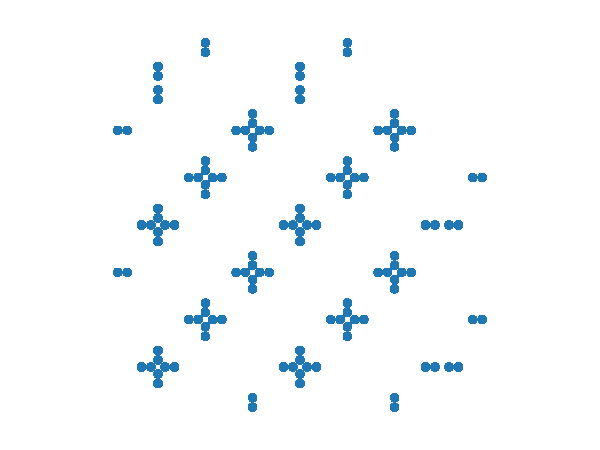
\includegraphics[width=0.5\linewidth]{../Figures/pegasus.pdf}
    \caption{A graph of 144 qubits in a D-Wave QPU, using their Pegasus topology. Qubits are represented by nodes, and couplers by edges.}
    \label{fig:pegasus}
\end{figure}

The qubits and their couplers define what can be seen as an energy landscape. Different combinations of qubit spins will have different energies, with the lowest energy state being the solution to the problem. A solver (or ``sampler'') attempts to characterise the shape of the energy landscape using a random range of input, and returns a number of samples with the lowest energy states. Note that the ``true'' ground state cannot be guaranteed; it could be part of the returned sample set, or may not even be found at all. It is the parameters of the annealing process that can reduce local minima and increase the likelihood of finding the ground state.

The full embedding process is often handled entirely by the QPU, done ``on the fly'' each time a problem is submitted. Fixed embeddings can be specified, but these require a priori knowledge of the specific QPU architecture. 

\section{Problem formulation}

Previous approaches to the automatic arrangement of music have relied on classical methods such as neural networks  or recursive classical algorithms  in order to produce arrangements that are musically sound. However, these methods are limited by the complexity of the problem and the need for extensive training data. In this study, a new approach to the automatic arrangement of music is proposed by applying quantum annealing.

It has been shown that the arrangement of music can be formulated as a combinatorial optimisation problem: given a set of musical phrases, each phrase can be assigned a binary variable and formulated into a Boolean satisfiability (SAT) problem, with variables assigned to clauses according to their compatibility. A valid solution would be an assignment of values such that the Boolean expression is satisfied, corresponding to the phrases included in the final arrangement . Phrases are chosen as the smallest unit of music instead of notes to best preserve important melodic lines and harmonies, which may sound dissonant or confusing if split up.

This paper focuses on the reduction of polyphonic (multi-part) music to a single monophonic part, where only one note can be played at a time. A reduction of this form would be relevant for arranging a string quartet for solo violin, for example, whilst still retaining all the important elements from across the instrument parts. This problem can be solved using a reduction of the SAT problem known as the maximum independent set (MIS) problem . Consider a set of musical phrases, each represented by a node $x_i$ in a graph $G$, with nodes connected by an edge if the phrases overlap. The aim is to find the largest subset of nodes such that no nodes within the subset are connected by an edge—the phrases corresponding to these nodes form the final arrangement. A formulation of this sort ensures that the reduction remains strictly monophonic, as no two chosen phrases play at the same time.

Denote $x_{v,i}$ to be a binary variable such that
\begin{equation}
    x_{v,i} =
    \begin{cases}
        1 & \text{if vertex $v$ is colour $i$} \\
        0 & \text{otherwise}
    \end{cases}
    \,,
\end{equation}

Proper vertex colouring constraints
\begin{equation}
    f(x)=A\sum_{v \in V}\left(1-\sum_{i=1}^{n} x_{v,i}\right)^2+A\sum_{(u,v) \in E}\sum_{i=1}^n x_{u,i}x_{v,i}
    \label{eq:MIS}
\end{equation}
where we take $x_i=1$ as the inclusion of that node in the solution set. The first term (penalty term) implements the independence constraint by increasing the energy by $A$ for each edge included, whilst the second term (objective term) is the quantity we are trying the minimise, the (negative) total number of nodes. $A$ and $B$ are known as Lagrange parameters, and can be chosen to balance the two terms accordingly. In this case, the condition $A>B$ must be satisfied, such that any penalty introduced by a node will outweigh its energy reduction.

\begin{figure}
    \begin{subfigure}[t]{0.5\linewidth}
        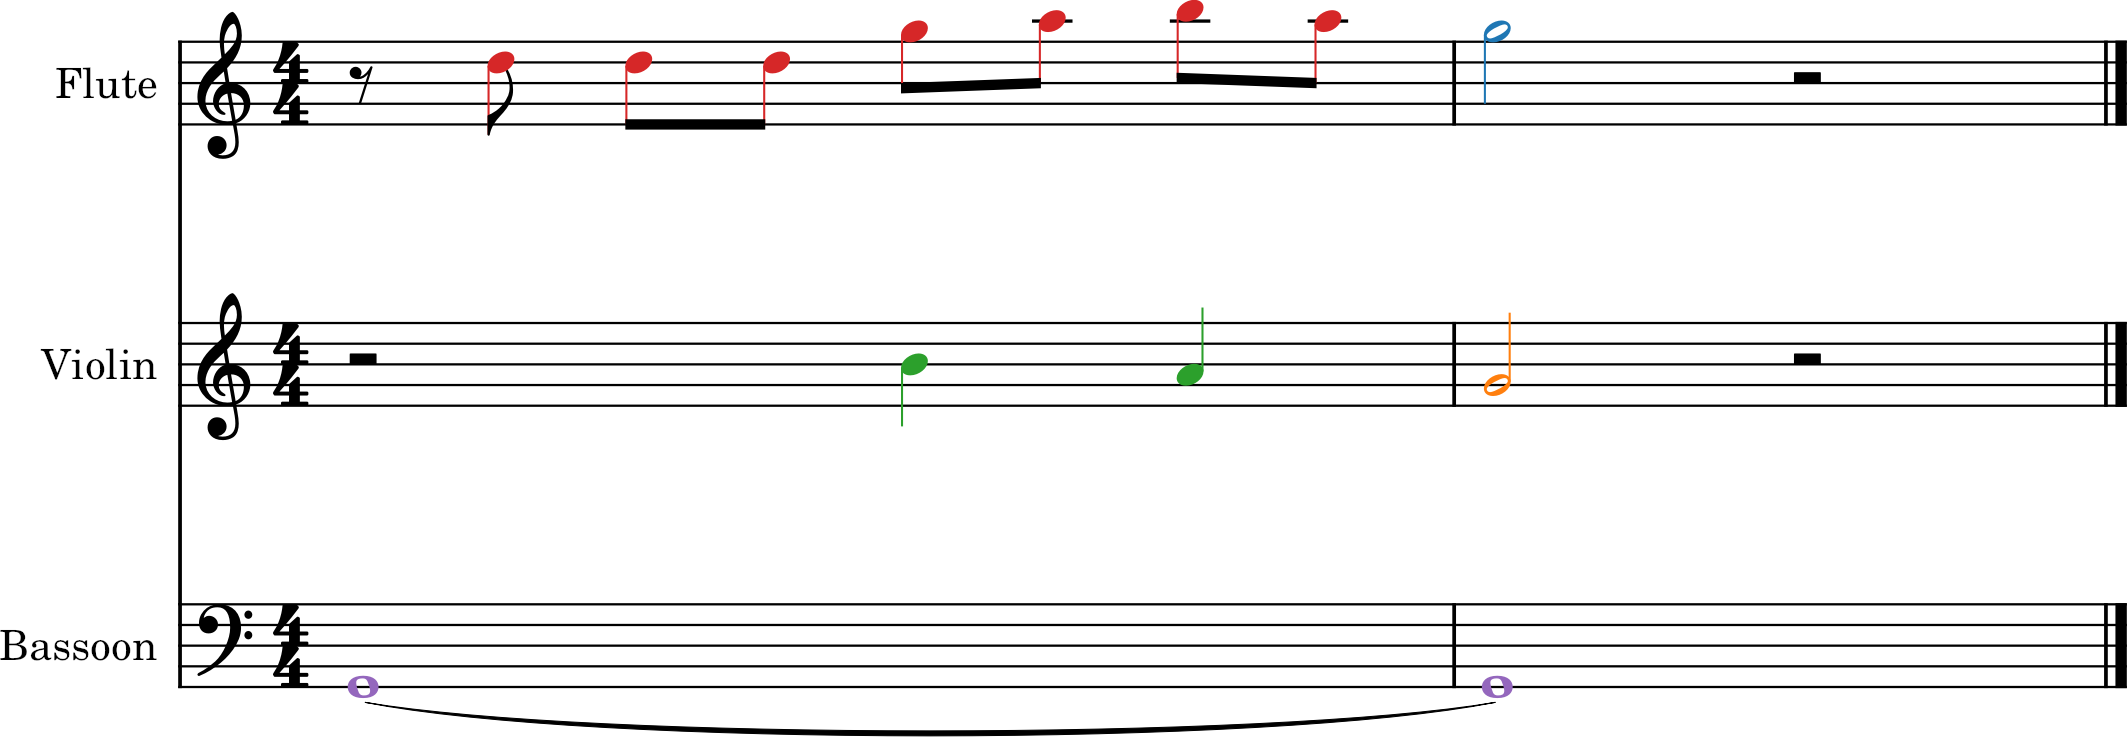
\includegraphics[width=0.95\linewidth]{../Figures/toy_trim-1.png}
        \caption{An example score of three parts, with each phrase coloured.}
        \label{fig:simple-excerpt}
    \end{subfigure}\hfill
    \begin{subfigure}[t]{0.5\linewidth}
        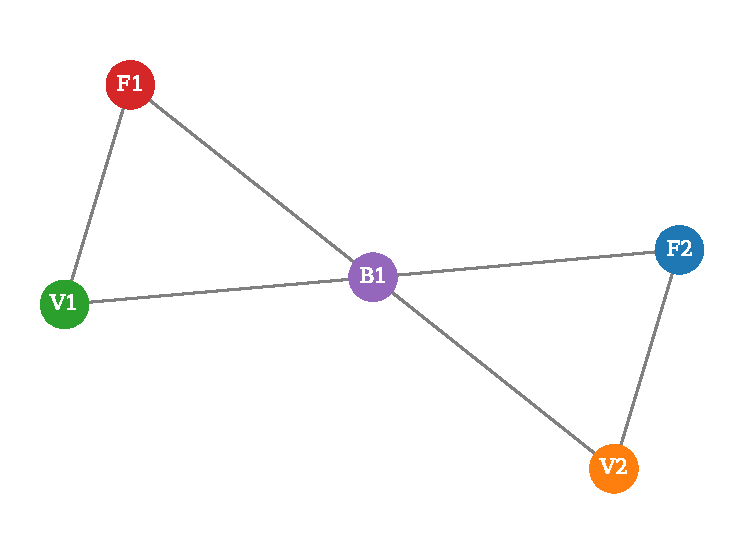
\includegraphics[width=0.95\linewidth]{../Figures/toy_graph.pdf}
        \caption{A graph of the score, with the colour of each node corresponding to its phrase, and edges connecting overlapping phrases.}
        \label{fig:simple-graph}
    \end{subfigure}
    \caption{A toy example demonstrating the construction of the problem graph. It is trivial to see that the maximal independent set contains two nodes.}
    \label{fig:toy}
\end{figure}

Final QUBO formulation:
\begin{align}
    f(x)=&A\sum_{v \in V}\left(s_v-\sum_{i=1}^{n} x_{v,i}\right)^2+B\sum_{(u,v) \in E}\sum_{i=1}^n x_{u,i}x_{v,i}\\-&C\sum_{v \in V}\sum_{i=1}^n W_vx_{v,i}-D\sum_{(u,v)\in E}W_{uv}\sum_{i=1}^n\sum_{j=1}^n x_{u,i}x_{v,j}-E\sum_{v \in V}\sum_{i=1}^n\theta(S_v-S_{\text{th},i})x_{v,i}
    \label{eq:weightedMIS}
\end{align}

$N_p * (n+1)$ logical variables in the BQM

% Physical implication of results
% Does code work? Comparison to literature, tests (IMPORTANT)

\section{Methods}

D-Wave Systems operates the first and only quantum annealer for commercial access, introduced in 2011 . All problems in this paper are run on the D-Wave Advantage quantum system, which uses their Pegasus architecture, with each qubit connected to 15 others (see Fig.\  ).
Interaction with the D-Wave QPUs is handled through their Leap quantum cloud service, which is used to submit problems to solvers. D-Wave provides an open-source software development package (SDK) of Python tools which allows users to translate problems into binary optimisation and create QUBOs for the QPU to solve.

Music can be represented by many digital formats, each with their own benefits—this study primarily uses MusicXML . This format focuses on the representation of standard sheet music, describing musical notes, rests, and other symbols, as well as the structure of the music, such as the arrangement of notes into measures (bars), parts, and scores. It is widely supported by music notation software, allowing translation of music to graphic (PNG, PDF) and audio (MIDI) formats. The Python module \verb|music21| provides extensive resources for manipulating, translating, and creating MusicXML files, allowing scores to be broken down and reconstructed as fit.

The reduction process begins by interpreting a MusicXML file of the original score. Embedded metadata within the score allows it to be broken down into its constituent parts, measures, and notes, as well as containing information about the instrumentation and structure. Each note is represented by a vector of features, such as pitch and duration, as well as its position within the wider piece, which can be measured as an offset (the number of beats from the start of the score).

To construct the problem graph, each individual part needs to be split into a sequence of musical phrases. The approach taken here is the local boundary detection model (LBDM) due to its easy implementation and good performance . The boundaries segmenting a part into phrases are identified using the degree of change between successive notes; larger differences between notes would show an increased likelihood of a boundary, exploiting the fact that the starts and ends of phrases are usually characterised by larger pitch or time intervals. Boundary strengths are calculated over two parameters, pitch and inter-onset interval (IOI), which is the difference between the starts of two notes. This is chosen over note duration as it is often more noticeable to the listener. The strength at note $i$ with parameter $x_i$ is given by
\begin{equation}
    S_i=x_i\times (r_{i-1, i} + r_{i, i+1})
    \label{eq:boundary-strength}
\end{equation}
where $r_{i, i+1}$ is the degree of change of a parameter between notes $i$ and $i+1$, given by
\begin{equation}
    r_{i, i+1}=\frac{|x_{i}-x_{i+1}|}{x_{i}+x_{i+1}} \,.
    \label{eq:degree-change}
\end{equation}
In this way, a note with a high boundary strength would signal the start of a new musical phrase. Each parameter's strength is normalised to the range $[0,1]$ according to the set of all strengths $S$ via
\begin{equation}
    S_i'=\frac{S_i-\min(S)}{\max(S)-\min(S)} \,.
    \label{eq:normalisation}
\end{equation}
Finally, to find the total boundary strength, the strengths of each parameter are summed with a weighting, using weights derived by trial-and-error ($0.3$ for pitch and $0.6$ for IOI) . If a note's total boundary strength surpasses a specified threshold, it is considered a boundary. Boundaries are always taken at the beginning and end of a score.

Once a list of boundaries is identified, the phrases are extracted by taking all the elements between subsequent boundaries. Each phrase is labelled according to the part it belongs to and its index within that part, allowing the phrases to be easily referenced and reconstructed into a new score once the optimisation is complete. To arrange the phrases into a graph, each phrase is checked against every other phrase for an overlap in time. Phrases are then represented by nodes, with edges connecting phrases that overlap.

The weight of each node is taken here to be the entropy of the phrase. Entropy can be seen as how much  information a variable contains; in this context, a phrase with a higher entropy would indicate a higher level of complexity, increasing the likelihood of it being more ``musical''. Maximisation of phrase entropy would then result in the creation richer arrangements. For a discrete random variable $X$ with a probability distribution $P(X)$, the Shannon entropy is defined as
\begin{equation}
    H(X):=-\sum_i P(x_i)\log_2 P(x_i)
    \label{eq:entropy}
\end{equation}
where each $x_i$ is a possible value of $X$ and ${\sum_i P(x_i)=1}$. In this context, the random variable is a musical note, considering its possible values both in terms of pitch and rhythm.

Pitch entropy is calculated by considering the distribution of pitches in a phrase. The probabilities of each pitch $x_i$ can be found by
\begin{equation}
    P(x_i)=\frac{n_i}{N}
    \label{eq:pitch-prob}
\end{equation}
where $n_i$ is the number of times pitch $x_i$ appears in the phrase and $N$ is the total number of notes in the phrase. A phrase with a greater variety of pitches (and thus greater entropy) will likely be more ``interesting'' in the final arrangement.
Rhythm entropy is calculated in a similar way, but considering the duration of the note instead. This is also calculated using Eq.\ \ref{eq:pitch-prob}, but instead considering $x_i$ as possible duration values.
The total entropy of a phrase is then the sum of the pitch and rhythm entropies.

Once the graph is formed, the weighted MIS QUBO can be constructed via Eq.\ \ref{eq:weightedMIS}, the Lagrange parameters chosen, and sent to the D-Wave QPU to be solved. The lowest energy solutions returned are sets of nodes that are not connected by edges, whilst maximising their total weighting. The qubits are then matched back to their corresponding phrases, which are reconstructed into a new score, the final reduction.

\section{Results}

The method was tested on an excerpt of (Haydn), taken from a MusicXML file in the public domain. This piece is ?? bars long and consists of four monophonic parts. It was chosen for...

Fig.\ ?? shows the extraction of phrases from the Violin I part by the LBDM.

\begin{itemize}
    \item Phrase extraction graph
    \item 
\end{itemize}

The resulting graph constructed from these phrases consists of ?? vertices and ?? edges. The QUBO formulation according to Eq.\ ?? was then calculated from this graph, to be submitted to the quantum annealer.

The annealer used in this study was the D-Wave Advantage 4.1 blah blah, which has connectivity of blah blah allows creation and submission of problems via a Python SDK (software development kit).

A returned sampleset of solutions might look something like Fig.\ [HISTOGRAM]. In most cases it's the lowest energy solutions (leftmost bins) that we care about.

How sparse is the problem graph? $(nodes + edges)/nodes^2$

\subsection{Lagrange parameter analysis}

Lagrange parameters were tuned to fulfil the required constraints for a valid arrangement. Node constraint => duplicates (phrases duplicated across parts), edge constraints => overlaps (phrases that overlap played at the same time).

\begin{itemize}
    \item Lagrange parameter variations
    \item 2D surface plot?
    \item Compare to analytic derivation (reference for double value?)
\end{itemize}

Analytically, we can derive an equality that the Lagrange parameters must satisfy in order for the minimum of the function to fulfil the imposed constraints.
\begin{equation}
    A>2\max(W)+E
\end{equation}
where $\max(W)$ is the largest entry of the weight matrix.

\begin{figure}
    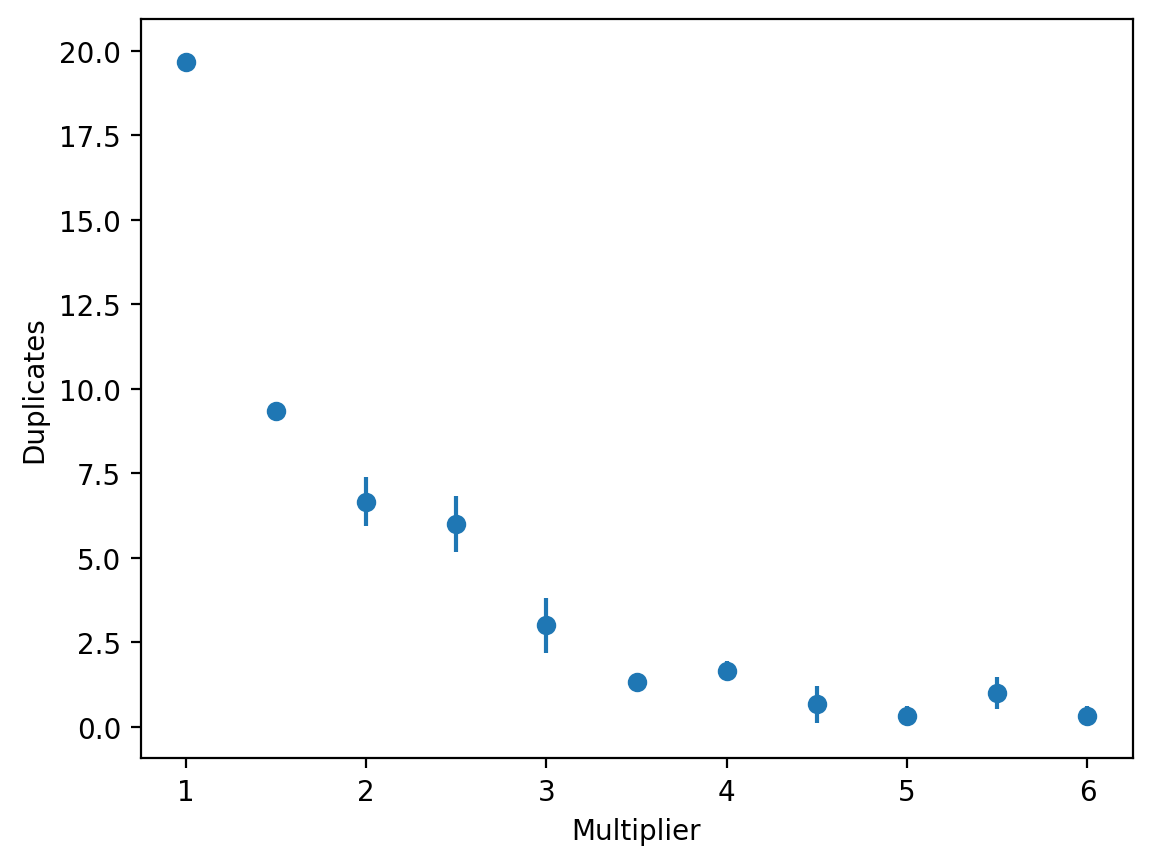
\includegraphics[width=0.5\textwidth]{node-constraint.png}
    \caption{Varying the node constraint Lagrange multiplier to ensure that each node is coloured at most once. Each QUBO was submitted three times for 1000 reads, with the mean and standard error calculated.}
\end{figure}

\begin{figure}
    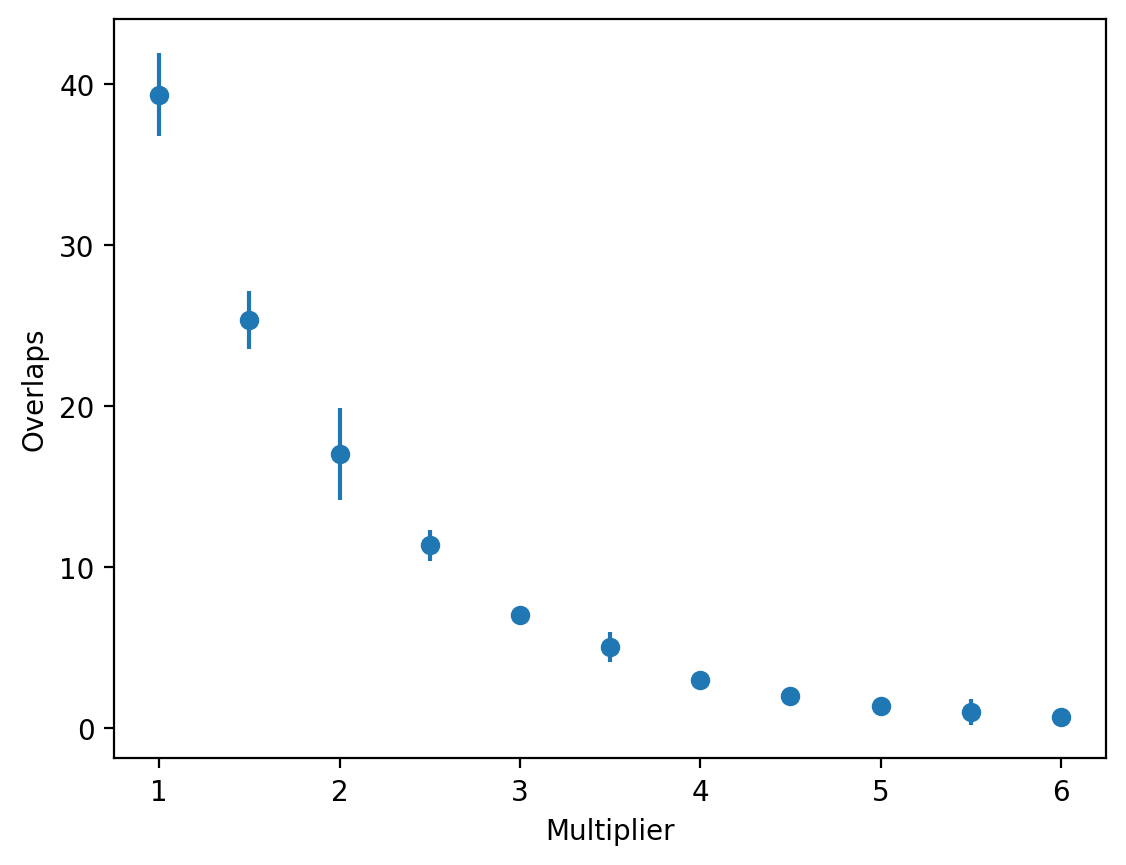
\includegraphics[width=0.5\textwidth]{edge-constraint.png}
    \caption{Varying the edge constraint Lagrange multiplier to ensure that no nodes of the same colour are connected.}
\end{figure}

\subsection{Solver configuration}

The configuration of solver used was also tuned: two parameters, chain strength and anneal time per sample.

Fit quadratic curve to chain strength plot to find minimum value of energy.

\begin{itemize}
    \item Chain strength analysis and explanation
    \item Anneal time analysis
\end{itemize}

\subsection{Comparison to classical algorithms}

Having tuned the Lagrange parameters and sampler configuration to give the lowest energy possible, we can compare the returned solutions to classical optimisation algorithms solving the same problem. D-Wave provides a selection of classical samplers that can return solutions to QUBO problems, two of which are used in this study. The steepest descent method blah blah. Simulated annealing, on the other hand, works very similarly to quantum annealing, but instead uses a "temperature" value to escape local minima. This method gives a more direct comparison.

Show energy against reads
Show total entropy against reads


\begin{itemize}
    \item Compare to classical for different problem sizes
\end{itemize}

\subsection{Scaling}

Scale two ways:

\begin{enumerate}
    \item Score length
    \item Number of instruments
\end{enumerate}

Compare lowest energy found for 

Phrases identified using the LBDM are shown in Fig.\  , alongside their calculated entropies according to Eq.\ \ref{eq:entropy} and their overlaps, represented by edges. A threshold value of $0.4$ was used, resulting in a total of 33 identified phrases, with 70 total overlaps. The calculated boundary strengths for the Violin 1 part can be seen in Fig.\ \ref{eq:boundary-strength}, with the identified boundaries summarised in Tab.\ . Many of the nodes form cliques of three or four vertices, that is, each node of the subset is connected to every other node. This can be expected, as often musical phrases across instruments will occur simultaneously, especially in small ensemble music such as this. Notably, there are also two disjoint cliques, subsets that are independent from the main graph. These can be seen as distinct musical ideas that are separated by rests from the other phrases (for example, the first two measures of the piece). A non-negligible number of phrases are calculated to have zero entropy—these are phrases identified as only having one note, and thus no variety in pitch or rhythm ($P(x_i)=1$).

The QUBO was calculated using Eq.\ \ref{eq:weightedMIS}, with Lagrange parameters $A=11.5$ and $B=1$. The value of $A$ was chosen to be twice the maximum node weight (phrase entropy) such that the penalty of choosing a node that introduces an edge into the solution would likely outweigh any possible benefit of its weighting. After submission of the QUBO to the D-Wave QPU, a sample set of solutions was returned, which can be seen in Fig.\  . Many solutions had degenerate energies—the lowest energy was -26.821803 with a degeneracy of 34 and zero chain breaks. These solutions used slightly different combinations of phrases to make the maximal independent set; this degeneracy is likely due to the high number of cliques, which only allows one node of the subset to be picked, and phrases with zero entropy, which do not change the final energy when interchanged. One of the lowest energy solutions can be seen in Fig.\  , with the nodes selected by the QPU highlighted. In this solution, none of the nodes are connected by edges, providing a valid monophonic arrangement. The musical score of this solution is shown in Fig.\  .

\section{Conclusions}

In the case of Beethoven's String Quartet No.\ 10, this method can be said to be successful in reducing the score to a single monophonic part. A sufficient number of phrases are identified to allow the key melodic lines to be picked out from each part, and the weighted MIS formulation results in a final arrangement that is not musically uninteresting. Here, only one solution was picked arbitrarily; if desired, each of the degenerate lowest energy solutions could be examined individually to isolate the one that is considered most ``musical'', safe in the knowledge that all of them are valid.

One advantage this method has over classical algorithms is that no training data is needed. Genetic and deep learning approaches require refinement of their models on large datasets, ``teaching'' what a valid arrangement looks like, which takes considerable time and resources. By using a QPU, these ``rules'' can effectively be encoded using constraints, such as the penalty term introduced into the QUBO; as long as these constraints are fulfilled, the QPU will always provide a feasible solution, without any knowledge of previous arrangements.

Another benefit is the solve time: for the problem graph shown in Fig.\  , the D-Wave QPU access time (the time taken to embed and solve the problem) is approximately 150 ms for 1000 reads. Compared to classical methods using a similar number of phrases, the quantum process is faster by at least one order of magnitude . For classical computers, the time taken to solve NP-hard problems increases exponentially with the problem size, so this speed advantage will only improve as the scores become more complex.

Future work would include testing this process on a wide range of pieces from different musical styles. Scores from different time periods (Baroque vs.\ Romantic, for example) have wildly different structures, and so the effectiveness of the LBDM could vary in identifying suitable musical phrases. The treatment of melodic lines between different ensembles, whether that be a string quartet or symphony orchestra, also varies, and the isolation of important melodic lines may become more difficult.

To that regard, the effect of LBDM parameters (pitch/IOI weighting, threshold) on phrase identification could be studied. Ideally, musical phrases should be fairly short and similar in length, to give the MIS algorithm the best chance in selecting the most interesting sections of the score. This would prevent important notes being hidden in long phrases with low entropy. Other boundary detection methods could also be tested, with their resulting identified phrases compared qualitatively.

Currently, no regard is taken to the exact instrumentation of the final arrangement. Different instruments have varying ranges of pitches that can physically be played; here, phrases have been chosen from across all the instrument parts (as seen in Fig.\  ), however, this does not mean that the final arrangement can be played by all the instruments as some notes may be unfeasible. Care needs to be taken to check the ambitus (pitch range) of chosen phrases and ensure that it falls within the desired instrument's range; if not, phrases can be transposed by octaves up or down without altering the melodies significantly.

The MIS formulation works well for reducing a score into a single polyphonic part, as the inclusion of a phrase within the final arrangement lends naturally to the binary variables used. However, a more useful application would be the ability to reduce a score to any fewer number of parts, whether that be multiple monophonic instruments (e.g.\ string quartet) or a polyphonic instrument (e.g.\ piano). To achieve this, the QUBO would need to be altered to allow some edges into the final subset. One suitable formulation would be a graph colouring problem: colouring the vertices of a graph $G$ with a set of $n$ colours such that no edge connects two vertices of the same colour. In this context, the number of colours would be the number of desired parts—after solving, each disjoint set of colours would become a monophonic part, the combination of which becomes the final reduction (in this way, the MIS problem can be seen as a colouring problem where $n=1$).

Although it can be argued that music cannot be objectively ``scored'', nonetheless, the quality of the produced arrangements needs to be judged in some way. One suggestion is that the ``goodness'' of music can only be measured via a Turing-like test, where human subjects are presented with a selection of both human- and computer-generated scores, and asked to categorise them . To this extent, a good measure of the arrangements produced by this method would be to compare them against popular arrangements of the same score composed by human professionals, via a series of blind trials. If the participants fail to identify the computer compositions from the human ones more often than random chance, then it can be said that the generated arrangements are of sufficiently good quality.

To conclude, this paper has shown the automatic reduction of music via quantum annealing. By formulating a score into a function to be minimised, the annealing process can identify parts of the original to become the final arrangement. An automatic process of this sort would be useful to a wide calibre of musicians, removing the time and skill barrier to produce such arrangements, whilst still retaining a sufficient level of quality, keeping music accessible to all. Just as science and business do already, it can be hoped that the arts take advantage of promising new technologies as well.

% References
\printbibliography[heading=bibintoc]

\clearpage

\section*{Scientific Summary for a General Audience} % 200 words

The arrangement of music by hand is usually a difficult and time-consuming process, requiring a deep understanding of musical theory and structure. This study aims to automate this process via quantum computing, a technique that relies on the use of qubits, which can exist in a superposition of states. A music score can be split up into a sequence of phrases by looking at how much adjacent notes differ from each other, and turned into a graph representation with nodes and edges, where each node is a phrase, and edges between nodes mean they overlap. This graph can then be sent to a quantum computer in order to select nodes according to a set of rules that determine the properties of the arrangement. Once the nodes have been selected, the corresponding phrases can be reconstructed to create the final score. Here, an excerpt of Beethoven's String Quartet No.\ 10 is reduced to a single part, suitable for a solo instrument.

\clearpage
\appendix
\section{Test appendix}

Start with an undirected graph $G=(V,E)$ and a set of $n$ colours, which represent the parts for which we are arranging, with each being an independent set. Denote $x_{v,i}$ to be a binary variable such that
\begin{equation*}
    x_{v,i} =
    \begin{cases}
        1 & \text{if vertex $v$ is colour $i$} \\
        0 & \text{otherwise}
    \end{cases}
    \,,
\end{equation*}
which requires $nV$ variables. The energy is
\begin{equation*}
    H = H_A + H_B + H_C + H_D \,.
\end{equation*}

Each vertex is coloured exactly once:
\begin{equation*}
    H_A = A\sum_{v \in V}\left(1-\sum_{i=1}^{n} x_{v,i}\right)^2
\end{equation*}

Vertices of the same colour are not connected by an edge:
\begin{equation*}
    H_B = B\sum_{(u,v) \in E}\sum_{i=1}^n x_{u,i}x_{v,i}
\end{equation*}

Maximise the weighting of selected vertices:
\begin{equation*}
    H_C = -C\sum_{v \in V}\sum_{i=1}^n W_vx_{v,i}
\end{equation*}

Maximise the weighting of included edges:
\begin{equation*}
    H_D = -D\sum_{(u,v)\in E}W_{uv}\sum_{i=1}^n\sum_{j=1}^n x_{u,i}x_{v,j}
\end{equation*}

It can be seen that for $n=1$ this reduces to the MIS problem. For a score with $p$ parts, it will be impossible to colour the graph exactly with $n<p$; the parameter $A$ should be small enough to allow for some vertices to remain uncoloured. The lowest energy solutions will return coloured independent subsets of $G$ that each represents a monophonic part of the final arrangement.

\end{document}